\documentclass{article}
\usepackage{ctex}  %使用宏包(为了能够显示汉字)
\title{自动驾驶中的车辆掉头问题}  %文章标题
\author{周宇昕\quad 徐圣泽\quad 郑天宇}   %作者的名称
\date{\today}       %日期
\usepackage{amsmath}
\usepackage{amssymb}
\usepackage{multirow}
\usepackage{longtable}
\usepackage{graphicx}
\usepackage{subfigure}
\usepackage[a4paper,left=25mm,right=25mm,top=25mm,bottom=25mm]{geometry}  
\newcommand{\enabstractname}{Abstract}
\newcommand{\cnabstractname}{摘要}
\newenvironment{enabstract}{%
	\par\small
	\noindent\mbox{}\hfill{\bfseries \enabstractname}\hfill\mbox{}\par
	\vskip 2.5ex}{\par\vskip 2.5ex}
\newenvironment{cnabstract}{%
	\par\small
	\noindent\mbox{}\hfill{\bfseries \cnabstractname}\hfill\mbox{}\par
	\vskip 2.5ex}{\par\vskip 2.5ex}
\usepackage{listings}

\begin{document}
	\maketitle
	\begin{cnabstract}
		本次要求解的是不同场景下的无人车调头问题。为解决这个问题,我们先通过建立一套完整的无人车驾驶体系模型,接着将这一体系模型代入各个问题中,最后相应地分别给出这些问题的求解结果。
		
		现实中的车辆往往是一个复杂的运动体,为更好地把握无人车的行驶过程,我们先将车辆转向过程进行模型化。在阿克曼转向模型的基础上,我们建立了车辆转向物理模型,选定了车辆的控制点为其后轴中点。此外,以后轴中点为轨迹点,我们确立了车辆各物理量之间的关系,将车自身量与轨道量紧密地联系在了一起。在该模型中,我们得到了以加速度和角速度即可控制车辆状态的结论。
		
		建立了车辆的转向物理模型,接着就是建立车辆的路径规划模型。在该模型中,我们以hybird A*算法为思想指导,确立了轨迹的组成与节点的选取。又根据题目条件设立了障碍物和曲率上的约束条件,并列出了含车道线项与路径光滑度项的目标函数。以路径经过节点为决策变量建立了整个路径的多目标规划模型。
		
		确立了路径规划后,我们转而结合前两个模型又建立了车辆控制优化模型。在该模型中,我们应用MPC模型的思想,根据题目要求,用路径拟合项、行驶时间项和加速度变化项组成了优化的损失函数。以各节点的加速度和角速度为决策变量,我们建立了车辆按既定路径控制的多目标优化函数。
		
		至此,已成体系的车辆驾驶模型已建立,我们将其运用于各场景中,可得到各场景下车辆的行驶路线。第一问是普通的调头,仅需注意车道线的影响。第二问我们从理论上计算了最窄调头范围并进行了验证。第三问加入障碍物项后,我们进一步改善了模型的表现形式,得到了不同障碍物存在可能性下的调头路线。第四问加入人行道后,我们判断调头必须要过人行道,相应地也给出了规划路线。第五问在移动障碍物情形下,我们加入障碍物的移动项,并调整规划和优化为实时性,尝试性地进行了运算。最后第六问我们分析了自己的算法并给出了改进的可能性意见。
		
		\par\textbf{关键字:车辆驾驶模型、hybird A*算法、多目标规划、MPC模型} 
	\end{cnabstract}
	
	\newpage
	\section{基本假设}
	\begin{itemize}
		\item[(1)]车辆运动时只考虑其运动学模型,而不考虑一切动力学因素;
		\item[(2)]无人车在行驶时,不存在一切如翻车、重心不稳等意外情况;
		\item[(3)]路面平缓,可提供车辆行驶所需的静摩擦力,车辆可在路面安全行驶;
		\item[(4)]无人车在转弯时保持匀速运动;
		\item[(5)]车辆前后左右对称,即前轮与后轮相对于车头、车尾的距离相同;
		\item[(6)]无人车具有自我感知与定位的能力。
	\end{itemize}	
	
	\section{变量声明及数据预处理}
	\subsection{变量声明}
	在解决本题的过程中,由于所设变量数较多,于是我们将多次用到的变量和符号名记录在下表中:
	\begin{table}[!h]
		\centering
		\caption{模型所需变量}
		\begin{tabular}{|l|l|}
			\hline
			变量 & 变量名 \\
			\hline
			轨迹点$t$时刻$x$坐标& $x(t)$\\
			轨迹点$t$时刻$y$坐标& $y(t)$\\
			轨迹点坐标&$z$\\
			轨迹点$t$时刻速度方向与$x$正半轴夹角& $\varphi(t)$\\
			轨迹点$t$时刻速度& $v(t)$\\
			曲率半径&$R$\\
			曲率 &$\kappa$\\
			轴距 &$L$\\
			方向盘转角&$\delta_r$\\
			方向盘角速度&$\omega_r$\\
			车辆转向所用总时长 &$T$\\
			障碍物(车道线)坐标 &$o$\\
			距离阈值 &$d$\\
			节点个数 &$N$\\
			规划目标项 &$P$\\
			规划权重系数 &$w$\\
			优化目标项 &$J$\\
			优化权重系数 &$\eta$\\
			临界宽度 &$Q$\\
			\hline
		\end{tabular}
	\end{table}

	\newpage
	\subsection{数据预处理}
	\begin{table}[h]
		\centering
		\caption{地图模型坐标点}
		\begin{tabular}{|c|c|c|c|c|c|c|c|}
			\hline
			\multicolumn{2}{|c|}{A} & \multicolumn{2}{c|}{B} & \multicolumn{2}{c|}{C} & \multicolumn{2}{c|}{D}    \\ \hline
			x          & y          & x         & y          & x         & y          & x            & y          \\ \hline
			15.35      & 0          & 3.67      & 16.15      & 7.15      & 16.15      & 11.15        & -0.35      \\ \hline
			15.35      & 32.19      & 3.67      & -0.31      & 7.15      & -0.31      & 11.15        & 15.89      \\ \hline
			0          & 32.19      &           &            &           &            & 10.63        & 15.89      \\ \hline
			0          & 0          &           &            &           &            & 10.63        & -0.35      \\ \hline
			\multicolumn{2}{|c|}{E} & \multicolumn{2}{c|}{F} & \multicolumn{2}{c|}{G} & \multicolumn{2}{c|}{初始位置} \\ \hline
			x          & y          & x         & y          & x         & y          & x            & y          \\ \hline
			15.43      & 18.09      & 0.14      & 13.29      & 7.78      & 24.22      & 13.57        & 4.96       \\ \hline
			15.43      & 20.84      & 0.14      & 8.4        & 7.78      & 16.22      &              &            \\ \hline
			0.46       & 20.84      & 5.14      & 8.4        & 9.68      & 16.22      &              &            \\ \hline
			0.46       & 18.09      & 5.14      & 13.29      & 9.68      & 24.22      &              &            \\ \hline
		\end{tabular}
	\end{table}
	\begin{figure}[!h]
		\centering 
		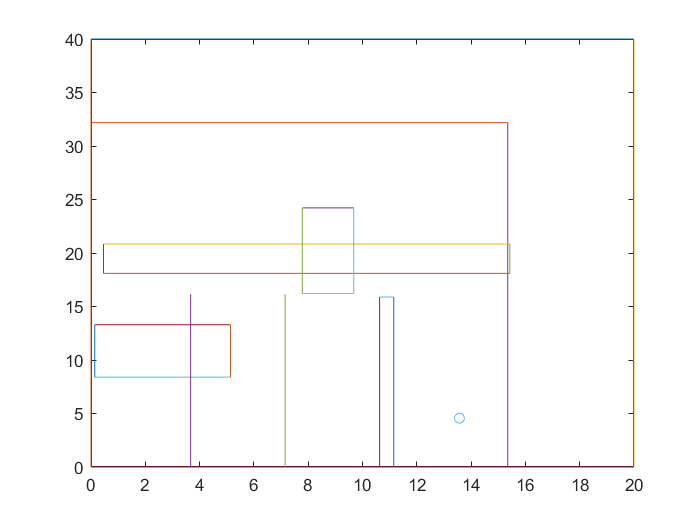
\includegraphics[width=0.6\textwidth]{primitiveposition.png}	
		\caption{初始时刻位置}
	\end{figure}

	\section{模型建立}
	\subsection{车辆转向物理模型}
	\subsubsection{阿克曼转向模型}
	实际问题中的车辆运动往往牵涉了很多量的变化,其运动是复杂的。而在我们控制车辆转向时,我们需要把现实复杂的车辆运动进行一定的简化。为此我们引入了研究无人车控制时常用的阿克曼转向模型,并以此为基础建立我们的车辆转向物理模型。阿克曼转向模型的示意图如下:
	\begin{figure}[!h]
		\centering 
			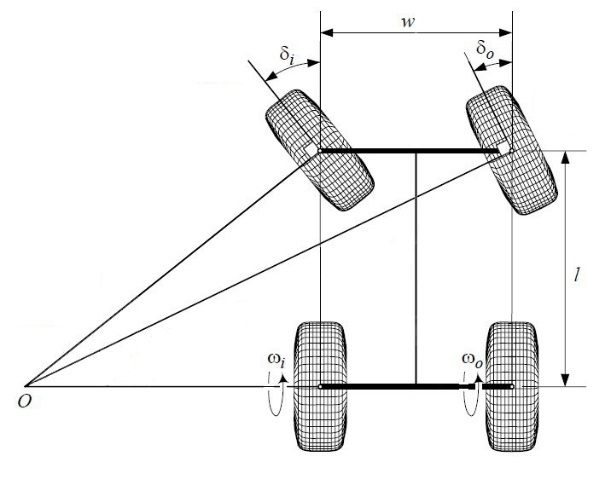
\includegraphics[width=0.4\textwidth]{阿克曼转向模型.png}	
			\caption{阿克曼转向模型}
	\end{figure}
    
    该汽车模型的建立是基于以下假设:
    \begin{itemize}
    	\item[(1)] 车辆在垂直方向的运动被忽略,也就是说我们描述的车辆是一个二维平面上的运动物体(可以等价于站在天空中的俯视视角)
    	\item[(2)] 转向时车辆的后轮不动,为制动轮;车辆仅由前轮控制转向
    	\item[(3)] 可以控制车辆前轮两轮的转角不同
    \end{itemize}

    由其模型推导出的基本公式为:
    \begin{equation}
    	\cot \delta_{i}-\cot \delta_{0} =\frac{w}{l}
    \end{equation}
    ($\delta_{i}$表示左前轮转角,$\delta_{0}$表示右前轮转角,$l$表示前后轴距,$w$表示前轮间距)
    
    由于以上模型中所用的一些物理量在本题并不适用,所以之后我们建立的模型会在该阿克曼转向模型的基础上进一步简化,从而得到本题情形下适用的关于车辆转向的物理方程。
    
    \subsubsection{控制点的选取}
    在本次题目中,控制点的选取是个至关重要的问题。由题目要求已知,控制点事先选定,位于无人车车身对称轴上一点。行驶时,控制点的位置会与轨迹点相重合,控制点处的速度方向将与轨迹点的方向角一致。因而只有确定了控制点,我们才能确定整辆车运动的轨迹,从而才能确立车辆运动的物理方程。
    
    而基于以上的阿克曼转向模型,控制点选取的答案呼之欲出。那便是车辆车轮后轴的中点。由于我们假设后轮不动,而前轮转动。所以在车辆中轴线上,只有后轴中点这一点上的速度方向与中轴始终保持一致,其余点在转向时的速度方向都会与中轴形成一定夹角。在该夹角不确定情况下,其余点作为轨迹点得到的位置与速度方向并不能确定整个车的位置与朝向。而后轴中点显然是可以做到这点的,那它就可以确定代表轨迹点,符合我们本题的要求。所以,在后续文章内容中,我们都以后轴中点作为控制点(轨迹点),以其位置和速度方向代表整辆车的运动,并建立起相关的物理方程。
    
    \subsubsection{物理方程的建立}
    确立了控制点(轨迹点)后,我们对于原有的阿克曼转向模型进行进一步改进,建立起我们应用于本题的车辆转向物理模型。在该模型中,我们把前后轮的运动都聚焦于中轴上的点,以前轴中点相对于轴的速度转向代表前轮的转向角度(将两轮视为一体,转角相同,这是进一步的假设),标示出相应的轨迹量与物理量,具体的示意图如下所示:
   \begin{figure}[!h]
    	\centering 
    	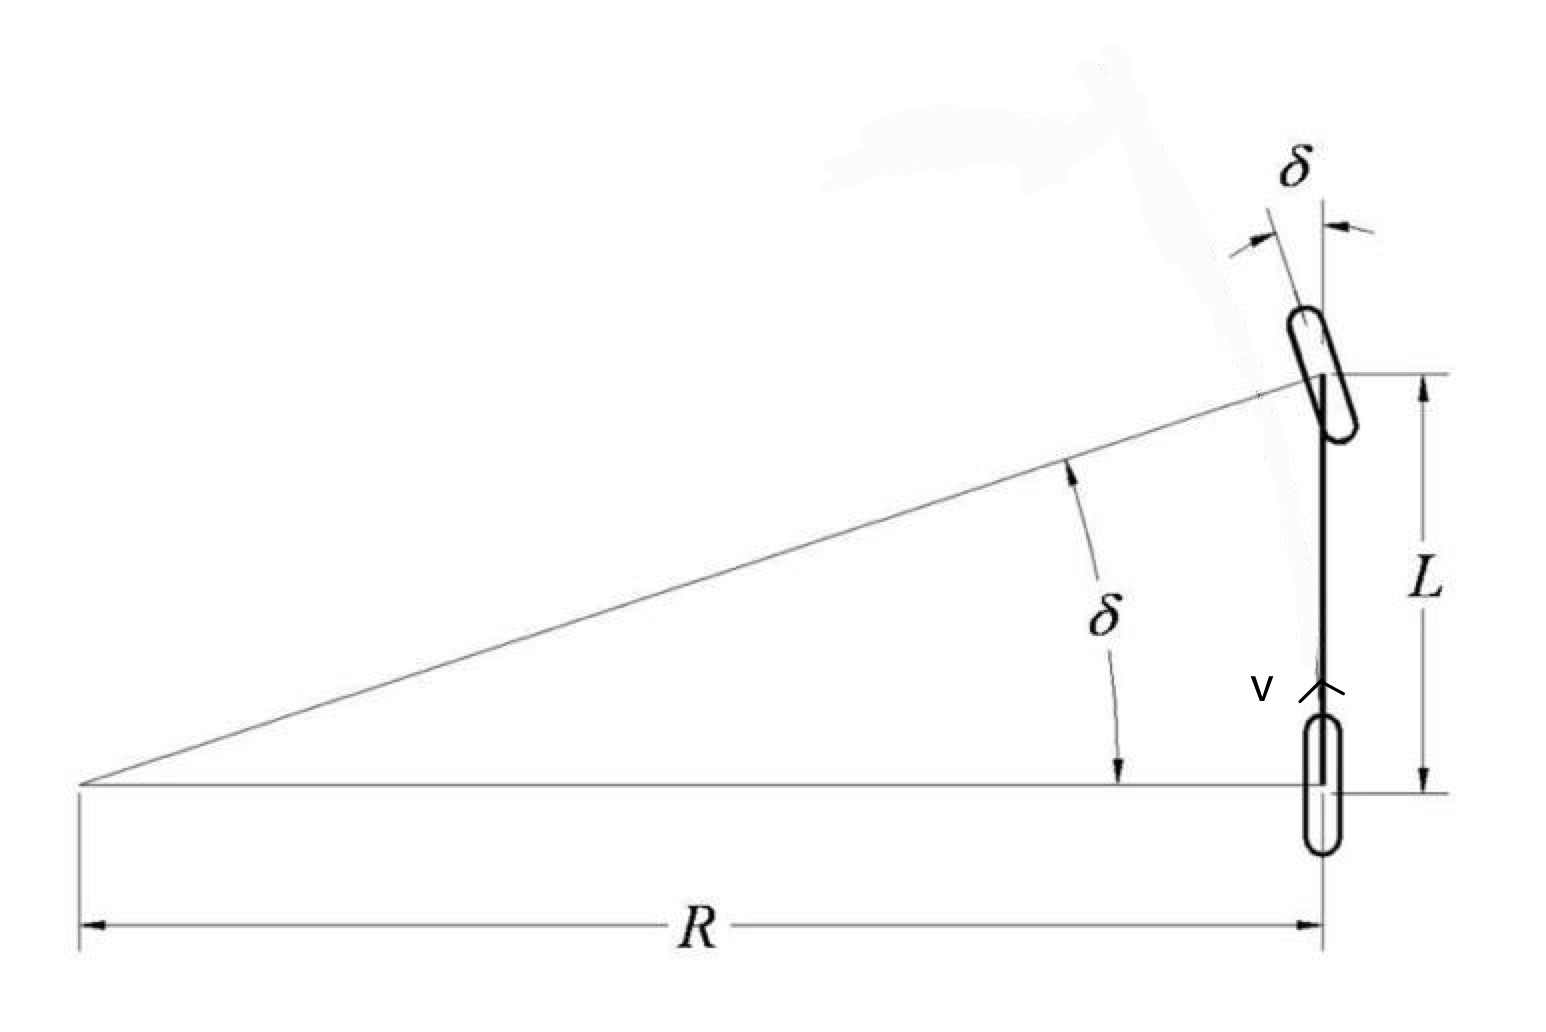
\includegraphics[width=0.4\textwidth]{车辆转向物理模型示意图.jpg}	
    	\caption{车辆转向物理模型示意图}
    \end{figure}

    用$(x(t),y(t),\varphi(t),v(t))$代表$t$时刻轨迹点的位置和速度,其物理关系方程如下所示:
	\begin{equation}
		\left\{
		\begin{aligned}
			x'(t)&=v(t)\cos\varphi(t)\\
			y'(t)&=v(t)\sin\varphi(t)\\
			\varphi'(t)&=\frac{v(t)}{R}\\
			v'(t)&=a(t)\\
		\end{aligned}
		\right.
	\end{equation}
    
    而从几何关系上进行分析,我们引入前轮转角$\delta$及其角加速度$\omega$,又可以得到关系式
    \begin{equation}
    	\delta'=\omega
    \end{equation}
	\begin{equation}
		R=\frac{L}{\tan\delta}
	\end{equation}
    
    又基于曲率半径$R$的表达式,可得
    	\begin{equation}
    	\varphi'(t)=\frac{v(t)\tan\delta}{L}
    \end{equation}
    而在本题中,前轮转角和角加速度实际上都由方向盘控制,所以我们又可以建立关系式:
	\begin{equation}
		\delta_r=16\delta,\omega_r=16\omega
	\end{equation}

    其中以上各物理量的限制关系为:
    \begin{equation}
    	-5m/s^2\leq a \leq 3m/s^2,\delta_{r} \leq 470^\circ, \omega_{r} \leq 400^\circ/s,L=2.8m
    \end{equation}

    那么其实确立了加速度$a$与角加速度$\omega$随时间的变化,就可以确立其他一切描述车辆运动的物理量,并且在这些量变化的前提下,车辆的轨迹、转动角度都是连续变化的,唯一剩下还需要考虑的就是轨迹的曲率$\kappa$。由物理关系式
	\begin{equation}
		\kappa=\frac{1}{R}=\frac{\tan\delta}{L}
	\end{equation}

    由车辆条件限制,$\delta\leq 470^\circ/16\approx 29.4^\circ$,则曲率$\kappa\leq \tan(29.4^\circ)/2.8\approx 0.201$,所以从车的控制原理上来说,轨道的曲率是始终会满足不高于0.205的要求的。相应地,车也有一定的转弯半径限制,其最小转弯半径$R\geq 1/0.201\approx4.97(m)$,这样的分析将帮助我们解决后续的问题。
    \subsection{车辆路径规划模型}
    以上部分是根据物理原理建立的车辆转向的物理模型。而在实际转向过程中,车辆行驶的前提是它已经形成了初步规划的路径。这就要求我们根据车辆行驶时的具体路况确立它的路径,这就是下面要建立的车辆路径规划模型,只有确定了大致的路径,接下来才能真正地控制车辆按规划路径去行驶。
    
    在建立我们的车辆规划模型时,我们将借助现有该领域比较先进的hybird A*算法的思想来帮助建立规划中相应的目标函数。
    
    \subsubsection{hybird A*算法}
     hybird A*算法主要用来解决在无人车有充分感知和定位能力情况下的路径规划问题。它能够在线重新规划生成障碍物地图,并且能够在未知环境中行驶。相较于同类的其他算法,该算法生成的路径足够光滑且能够满足无人车运动时的非完整约束。它的优点就在于可以在连续坐标下进行启发式搜索,并能够利用一定的共轭梯度下降法对生成的路径进一步改进,使其至少满足局部最优。我们的规划模型即基于该算法的思想。
     
    hybrid A* 在线路精度一致的前提下(对应某一小段时间)通常使用三种控制动作:最大左转,最大右转,直行来生成路径,因此该路径通常是一些受车辆转弯半径约束的圆弧和直线。在本题中由于车辆前轮转角要求是连续变化的,所以适当时候也会根据车辆的最大转角要求在路线中加入一定的衔接曲线。
    \subsubsection{目标函数的确立}
    车辆路径的确立本质上是一个规划问题,因而也有规划约束项和目标函数的确立。根据题意,本题条件下路径规划的约束主要体现在:
    
    \textbf{1.障碍物。}题目要求按轨迹行驶时,无人车车身任何点不得与任何障碍物或者掉头区域边界发生碰撞,且与障碍物至少保留一个最小安全距离,一般不小于30cm。这就是对于路径规划的一个重要约束条件,数学表达式可列为:
        \begin{equation}
    |z_{i}-o_{i}|\geq d_{obs}
    \end{equation}
	其中$z_{i}$为路径节点坐标(车上任意点的坐标也考虑在内),$o_{i}$为最近障碍物的坐标,$|z_{i}-o_{i}|$代表它们之间的距离,$d_{obs}$为与障碍物距离的阈值,在本题情况下即为30cm。

    \textbf{2.曲率。}基于物理模型的讨论,受车辆本身参数条件的限制,轨迹的曲率也存在着一定限制,即不得超过0.201。这是对于路径规划的一个重要约束条件。不同节点下,$\Delta z_{i}=z_{i}-z_{i-1}$,$\Delta\varphi_{i}=\cos^{-1}\frac{z_{i}*z_{i-1}}{|z_{i}||z_{i-1}|}$,瞬时曲率$\kappa=\frac{\Delta \varphi_{i}}{|\Delta z_{i}|}$。则关于各节点瞬时曲率的约束条件可列为:
   \begin{equation}
   	\frac{\Delta \varphi_{i}}{|\Delta z_{i}|}\leq \kappa_{max}
   \end{equation} 
	其中$\kappa_{max}$即为最大曲率限制,在本题中即为0.201。

    有了基本的规划约束条件,接下来就是确立规划的目标函数。根据题意,在确定路径时,我们还需要尽量减少不必要的压车道线行驶,同时路径的光滑性要足够的好,以保证正式行驶时各变量能连续变化,曲线充分对应。这即给规划定下了两个目标,这是一个多目标规划模型。以$P$代表最终的目标函数量,$P_{lan}$代表有关车道线的目标量,$P_{smo}$代表有关光滑度的目标项,其具体函数形式分析如下:
    
    \textbf{1.车道线项。}由于要减少不必要的压车道线行驶,所以与障碍物时情况类似,同样以$o_{i}$代表离车最近的车道线的坐标,$z_{i}$为路径节点坐标(车上任意点的坐标也考虑在内),车道线项可以具体表现为
       \begin{equation}
     P_{lan}=w_{lan}\sum_{i=1}^{N}|z_{i}-o_{i}|
    \end{equation}
	其中$|z_{i}-o_{i}|$代表路径节点与对应车道线节点之间的距离,$N$为节点个数,$w_{lan}$则是对于多目标规划所需的权重系数,应根据目标需求和实际情况加以确定。由于要减少压车道行驶,所以我们希望该项越大越好,在目标函数中为max。

    \textbf{2.光滑度项。}我们的目标需要让路径尽量光滑,关于这一点,我们用每个节点之间位移向量的差值的平方来表示,光滑度项的具体表现形式为:
           \begin{equation}
    	P_{smo}=w_{smo}\sum_{i=1}^{N-1}(\Delta z_{i+1}-\Delta z_{i})^2
    \end{equation}
	其中$w_{smo}$是对于多目标规划所需的权重系数,也应当根据目标需求和实际数大小情况加以确定。由于要尽量光滑,所以我们希望该项越小越好,在目标函数中应取为min。
	
	基于以上的讨论,在最终的目标函数中,应是两者的结合。由于二者关于大小取向不同,以max为基准,我们的目标为
	\begin{equation}
	max\quad P=P_{lan}-P_{smo}
	\end{equation}
	至此,我们以hybird A*算法为思想支撑,根据题目条件列出了路径规划的约束项和目标函数,以路径节点为决策变量,建立起了整个路径规划模型。根据该模型,我们可以尝试为无人车在具体行驶环境中找到一条相对优越的路径。
	\subsection{车辆控制优化模型}
	由车辆路径规划模型得到了车辆期望行驶的路径,那么接下来就要解决如何根据车辆转向的物理模型来控制车辆尽量沿着该路线行驶,并同时能期望满足题目的要求。为此,我们参阅网上资料,在这个环节上决定引入模型预测性控制(MPC)理论,以追求短时间间隔内车辆的优化控制。于是,在MPC理论的基础上,我们决定构建适用于本题情形的车辆控制优化模型。为此,我们需要构建优化目标函数,而由于题目要求的多样性,这同样是一个多目标优化问题。我们记最终的优化损失函数和其各项为$J$。

    由车辆的物理模型我们已知,$(a,\omega)$决定了一辆车之后一段短时间$dt$内的行驶情况(假设这二者在这相当短的时间内不变)。而又由车辆路径规划模型我们得到了车辆的期望行驶路径,在其中我们可以选取适当的节点,通过真实路径与预期路径的对比来判断控制是否妥当。因而路径的契合性是优化损失函数中的第一项,我们用$J_{L}$来代表,其具体表现形式可写为:
    \begin{equation}
    	J_{L}=\eta_{L}\sum_{i=1}^{N}(z_{i}-z_{ref,i})^2
    \end{equation}
	其中$N$为选取的节点个数,$z_{i}$为车辆控制的节点坐标,$z_{ref,i}$为与之对应的参照规划路线的节点坐标,$\eta_{L}$为优化的权重系数,应根据具体情况提前确定给出。作为优化损失函数一部分,它应当取min。

	路径契合是对于车辆控制的基本需求,而分析题目,我们发现在本题的车辆控制中还应考虑具备尽可能舒适的驾乘体感,以及具备尽可能高的通行效率,这两项也是我们在优化中需要考虑的优化项。首先关于通行效率,因为路线已定,其相关量可以通过整个转向调头过程所用总时间$T$来衡量。记优化量为$J_{T}$,
	\begin{equation}
		J_{T}=\eta_{T}T
	\end{equation}
	其中,$\eta_{L}$为优化的权重系数,应根据具体情况提前确定给出。作为优化损失函数一部分,我们希望通行时间越短越好,同样取min。
	
	最后,我们考虑乘客要具备尽可能舒适的驾乘体感,这意味着车辆在运行时不能频繁变速,由于每个节点都有对应的加速度$a$,即要求不同节点间的$a$值不能相差过大。记该优化量为$J_{A}$,它的表现形式可写为:
    \begin{equation}
	J_{A}=\eta_{A}\sum_{i=1}^{N-1}(a_{i+1}-a_{i})^2
	\end{equation}
	其中,$\eta_{A}$为优化的权重系数,应根据具体情况提前确定给出。作为优化损失函数一部分,驾乘体验好,意味着该项取min。

	所以综上,我们大致确立了该控制优化模型中的优化损失函数的表现形式,应满足:
    \begin{equation}
		min\quad J=J_{L}+J_{T}+J_{A}
	\end{equation}

	以上便是我们根据本题建立的车辆控制优化模型。在车辆具体控制过程中,我们要将该优化函数始终放入关于$(a,\omega)$组合的考量中,从而最终确立合理的加速度与角速度关于时间的变化结果,并最终确立真实的车辆行驶路径。
	
	\newpage
	\section{问题求解及结果}
	根据以上建立的车辆路径规划和控制优化模型,代入具体的场景,运用一定的算法,我们可以分别求解第一问至第五问,并得到相应的结果。
	\subsection{第一问}
	第一问是最简单的调头模型,不存在障碍物项,车辆最后的路径规划如下所示,也能成功控制车辆运行该路径。
	\begin{figure}[!h]
		\centering 
		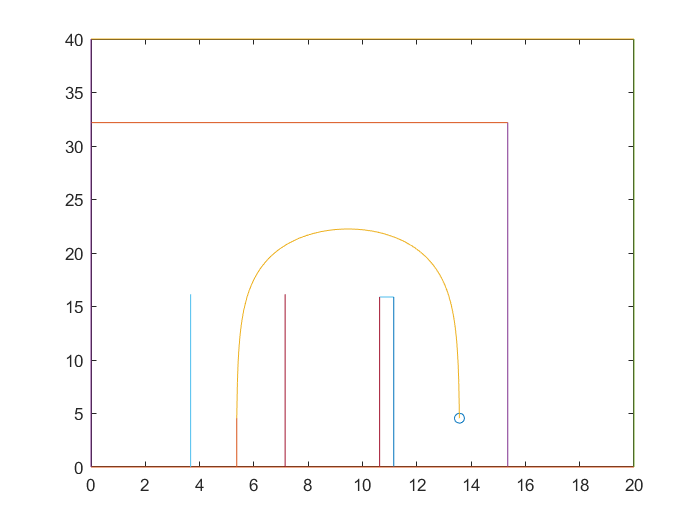
\includegraphics[width=0.6\textwidth]{problem1.png}	
		\caption{路线轨迹图}
	\end{figure}
	\subsection{第二问}
	从理论上来说,车辆转向时有最小转向半径的要求,$R_{min}=4.97m$,对于第二问的调头情形来说,由于中轴的方向角要转180$^\circ$,所以其转向的横向宽度至少为两个最小转向半径。此外,边界作为障碍物,有距离阈值的要求,车本身也带有一定的宽度,所以调头区域的临界宽度为
	\begin{equation}
		Q=2\times R_{min}+2\times d+w=2\times 4.94+2\times 0.3+2=12.54m
	\end{equation}
	因此,对于第二问,当区域宽度$\geq12.54m$时,车辆能够正常一次调头通过,而不足$12.54m$时无法直接通过,需要至少一次倒车。
	
	\subsection{第三问}
	在该问中,我们的调头需要考虑障碍物的各项因素。为此,在第一问已有的算法基础上,我们按照路径规划模型中的障碍物项加入相应的障碍物量,对算法进一步优化修改,最终得到了在障碍物F、G单独存在和同时存在情况下的最优调头路线,如下图所示:
	\begin{figure}[!h]
	\centering 
		\subfigure[一个障碍物1]{
		\label{Fig.sub.1}
		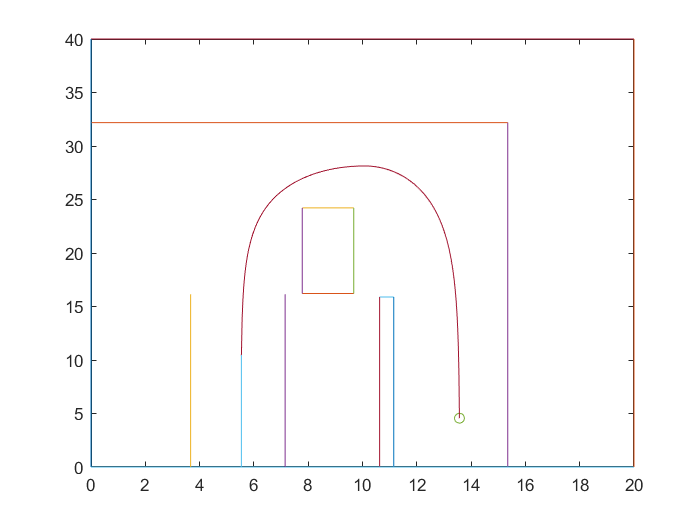
\includegraphics[width=0.3\textwidth]{p3一个障碍物1.png}}
	\subfigure[一个障碍物2]{
		\label{Fig.sub.2}
		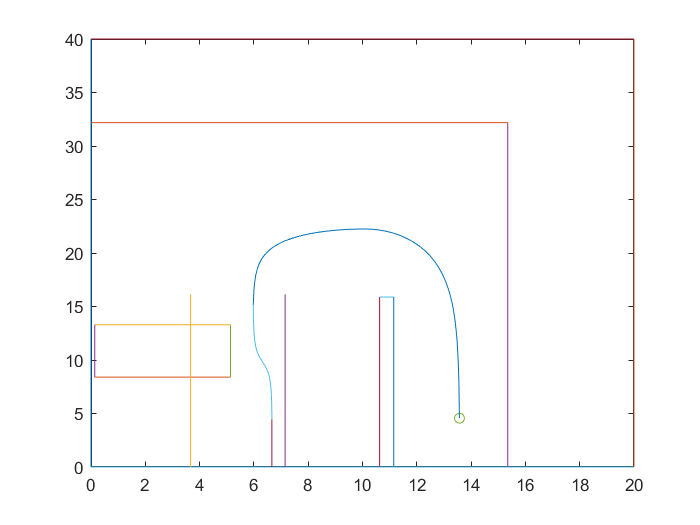
\includegraphics[width=0.3\textwidth]{p3一个障碍物2.png}}
	\subfigure[两个障碍物]{
		\label{Fig.sub.3}
		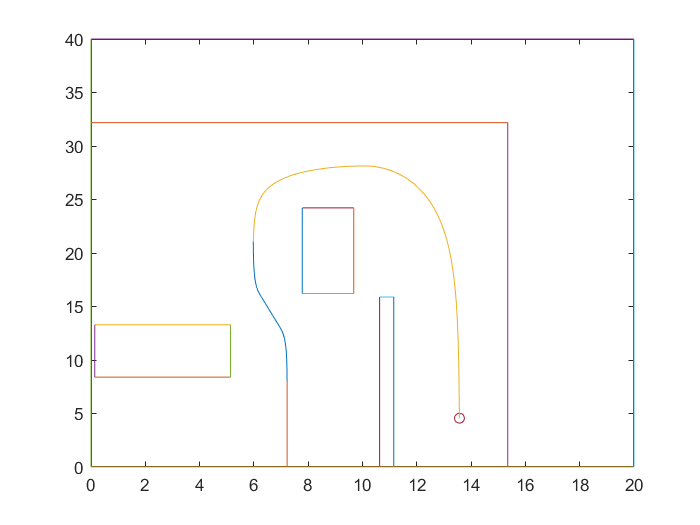
\includegraphics[width=0.3\textwidth]{p3两个障碍物.png}}
	\caption{路线轨迹图}
	\end{figure}

	\newpage
	\subsection{第四问}
	该问中,我们要考虑人行道的因素。这就要加入轨道中弧线开始时位置的约束方程,需要判断该位置是否合理。首先判断调头是否一定要完全穿过人行道,即开始转弯位置在人行道前。在尝试后,我们的算法告诉我们这不可能。所以,不论是否有障碍物,此时的转弯都需要在人行道后,这是一个新加的约束条件。在第一问和第三问的算法基础上,加入这个约束条件,我们得到的车辆调头轨迹如下图所示:
	\begin{figure}[!h]
		\centering 
		\subfigure[人行道和一个障碍1]{
			\label{Fig.sub.1}
			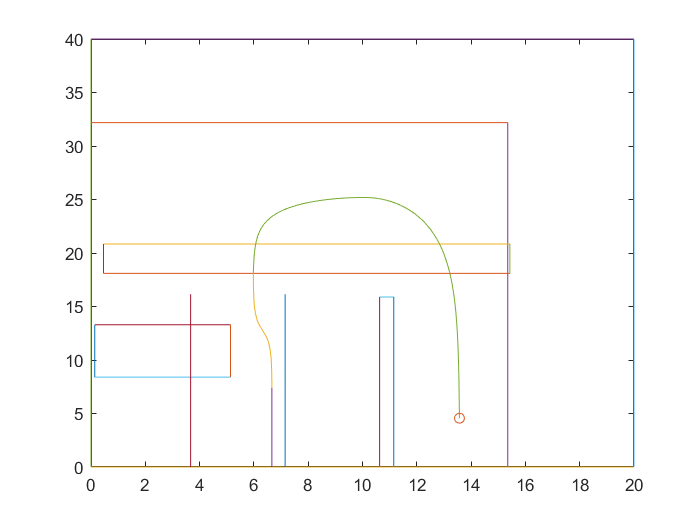
\includegraphics[width=0.4\textwidth]{p4人行道和一个障碍1.png}}
		\subfigure[人行道和一个障碍2]{
			\label{Fig.sub.2}
			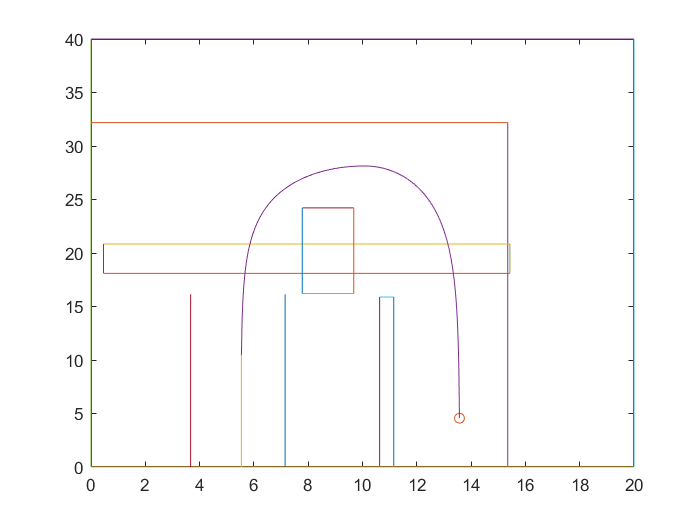
\includegraphics[width=0.4\textwidth]{p4人行道和一个障碍2.png}}
		\subfigure[p4只有人行道]{
			\label{Fig.sub.3}
			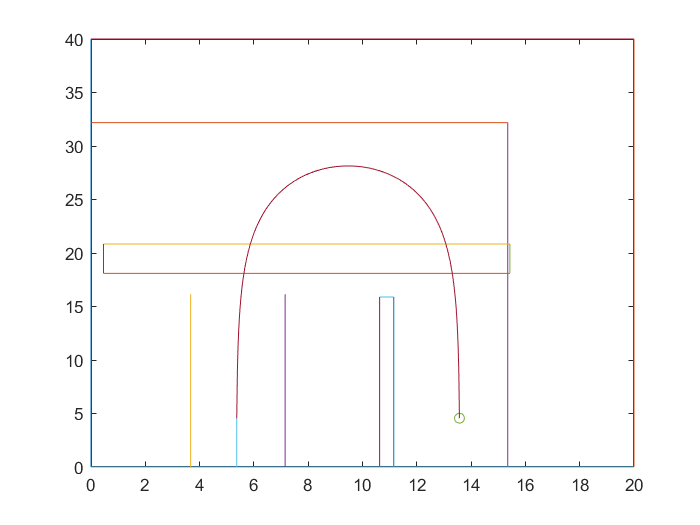
\includegraphics[width=0.4\textwidth]{p4只有人行道.png}}
		\subfigure[完整路况]{
			\label{Fig.sub.4}
			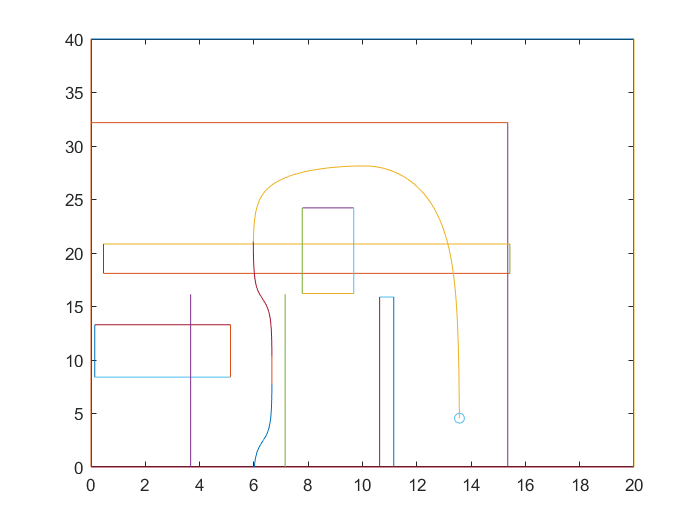
\includegraphics[width=0.4\textwidth]{p4完整路况.png}}
		\caption{路线轨迹图}
	\end{figure}

	\subsection{第五问}
	该问中,障碍物处于移动状态,所以在我们的路径规划模型中,在考虑障碍物时,我们要加入一系列有关其移动的变量。而同时,由于物体的移动,路径规划无法事先完成,而要在线变动,从而也会引起控制的优化也应是在线优化的。为此,在我们的模型中,我们将缩小区域搜索的范围和控制优化延续时间的范围,要倚靠不断运算和判断来实现。但可惜的是,我们的算法复杂度较高,在移动变化的情况下无法短时间在线地给出相对较好的结果。同时由于动画展现水平的限制,该问我们只能提出模型和算法改进的意见,而无法呈现出较好的结果。
	\subsection{第六问}
	在具体求解移动变化情况时,我们发现我们已有的算法复杂度较高,无法有效求解。许多情景在靠人工输入判断,耗时长,也缺少更多场景下的普适性。为在算法的求解成功率和耗时上进行优化,我觉得有以下几个方向可以拓展:一是尽力开拓遗传算法、蚁群算法等优越的启发式算法和机器学习相关算法在车辆模型求解上的应用;二是引入一些在线算法的思想,基于在线优化理论对模型的相关函数进行进一步改进;三是在数学理论上研究更有效的区域关系表现形式、物理方程表达形式等;四是建立相关的算法平台,可以根据车辆参数模拟仿真车辆的行驶过程,并在平台中可以不断检测、改进。
	\section{结语}
	在本题的探究过程中,我们建立了数学规划的模型,并针对不同要求设计了相应算法,总体而言可以较好地满足题目的要求,解决了相应的问题,并且有一定的实际应用价值。对于探究过程中出现的问题,我们也进行了分析并提出了相应的解决策略,但因为时间关系没有进行更深入的探讨,恳请批评指正!

	\begin{thebibliography}{10}  
		\bibitem{ref1}郭景华,胡平,李琳辉,王荣本,张明恒,郭烈.基于遗传优化的无人车横向模糊控制. 机械工程学报.2021.3.
		\bibitem{ref2}刘果.无人驾驶汽车转向控制方法及研究.硕士学位论文.2017.6.
		\bibitem{ref3}张琨.智能汽车自主循迹控制策略研究.哈尔滨工业大学博士学位论文.2013.9.基于遗传优化的无人车横向模糊控制
	\end{thebibliography}
	
\end{document}

